%%% DOCUMENT PREAMBLE %%%
\documentclass[12pt]{article}
\usepackage[english]{babel}
%\usepackage{natbib}
\usepackage{url}
\usepackage[utf8x]{inputenc}
\usepackage{amsmath}
\usepackage{titlesec}
\usepackage{graphicx}
\graphicspath{{images/}}
\usepackage{parskip}
\usepackage{fancyhdr}
\usepackage{vmargin}
\setmarginsrb{3 cm}{2.5 cm}{3 cm}{2.5 cm}{1 cm}{1.5 cm}{1 cm}{1.5 cm}

\setcounter{secnumdepth}{4}
\setcounter{tocdepth}{4}
\title{}								
\author{A Recommender System for News (RSN)}						
\makeatletter
\let\thetitle\@title
\let\theauthor\@author
\let\thedate\@date
\makeatother
\pagestyle{fancy}
\fancyhf{}
\rhead{\theauthor}
\lhead{\thetitle}
\cfoot{\thepage}

\titleformat{\paragraph}
{\normalfont\normalsize\bfseries}{\theparagraph}{1em}{}
\titlespacing*{\paragraph}
{0pt}{3.25ex plus 1ex minus .2ex}{1.5ex plus .2ex}
%%%%%%%%%%%%%%%%%%%%%%%%%%%%%%%%%%%%%%%%%%%%
\begin{document}
\tableofcontents
\pagebreak
%%%%%%%%%%%%%%%%%%%%%%%%%%%%%%%%%%%%%%%%%%%%
\renewcommand{\thesection}{\arabic{section}}
\section{Introduzione}
\subsection{Scopo Requirement Document}
 
 Lo scopo di questo documento è quello di fornire una documentazione il più dettagliata possibile riguardo le specifiche dei requisiti del progetto A Recommender System for News (RSN), sistema che fornisce una lista di news all’utente in base alle sue preferenze; le news proposte all’utente sono tutte prese dai tweet degli account Twitter di importanti testate giornalistiche. L’obiettivo finale è quello di realizzare una web app a cui chiunque possa registrarsi ed accedere per essere aggiornato sulle notizie riguardanti gli ambiti a cui è più interessato.
 
In questo documento verranno illustrate le features e altre informazioni riguardanti il progetto in modo da fornire una visione d’insieme del prodotto che vogliamo sviluppare.
 
 
\subsection{Scopo del progetto}

L’idea che sta alla base del progetto è quella di creare un’applicazione disponibile sul web a qualsiasi utente sia interessato a notizie giornalistiche che possono coprire diversi ambiti; lo scopo principale consiste nel mettere in evidenza notizie di determinate categorie (es. sport, politica, etc.) piuttosto che altre in base agli interessi dei diversi utenti. Per poter eseguire questa operazione è necessaria una fase di profilazione degli utenti che avverrà durante la registrazione all’applicazione.

La fase di sviluppo del progetto è stata suddivisa in due parti: crawler e algoritmo per l’analisi, l’indicizzazione e la raccomandazione delle news.
 
\subsubsection{Crawler} 

Questa parte riguarda la raccolta dei dati, che nel nostro caso sono rappresentati dalle news.

L’ambiente in cui andiamo a raccogliere i dati è il social network Twitter, grazie alle api-Twitter; più precisamente le news che scarichiamo sono prese dagli account di alcune testate giornalistiche che pubblicano quotidianamente nuove notizie

\subsubsection{Algoritmo}

Algoritmo per l’analisi, indicizzazione e raccomandazione delle news.

Questa parte riguarda l’analisi e l’elaborazione dei dati raccolti nella fase precedente; in particolare abbiamo effettuato operazioni di analisi e indicizzazione dei dati (preprocessing) ed in seguito abbiamo sviluppato l’algoritmo di raccomandazione in base alle preferenze degli utenti.


\subsection{Definizioni, acronimi, abbreviazioni}
\subsection{Riferimenti}
\subsection{Overview}


\newpage
\section{Descrizione Generale}

\subsection{Visione del prodotto}
\subsubsection{Ambito del progetto}

L’applicazione (RSN) si colloca nell’ambito di reperimento informazioni legate a news reperite da Twitter e può renderle visibili all’utente in base agli interessi di quest’ultimo. Il progetto è suddiviso in due parti: crawler delle news e metadati, e analisi tramite algoritmo di raccomandazione dei dati raccolti.

\subsubsection{Ambiente}

L’applicazione finale funzionerebbe in prima battuta su qualsiasi tipo di browser cosicché l’utente sia in grado di autenticarsi sul nostro sistema ovunque e con qualsiasi dispositivo. I dati che forniremo all’utente sono provenienti dagli account Twitter di alcune delle più note testate giornalistiche.

L’ambito di interesse è Twitter in quanto lo scopo del progetto è rendere disponibili i dati raccolti dal social network e a questo scopo sono necessarie le api-twitter per poter creare un crawler per raccogliere i dati.

L’applicazione finale funzionerebbe in prima battuta su qualsiasi browser. Cosicché l’utente abbia la possibilità di loggarsi ovunque e da qualsiasi dispositivo.

\subsubsection{Evoluzioni future}

Il primo passo sarà quello di implementare una maggiore fonte di notizie andando a raccogliere dati da fonti differenti da Twitter. L’evoluzione futura di questa webApp prevede la creazione dell’applicazione su piattaforme mobile come Android o IOS.


\subsubsection{Confronto con business-concorrents (altri modelli simili)}

Nello sviluppare la nostra idea per il NRS abbiamo notato una forte somiglianza per funzionalità e concetto base di funzionamento con il sistema Flipboard. Quest’ultimo presenta sia la profilazione dell’utente che la raccomandazione delle news in base alle preferenze ed inoltre l’aggregazione più fonti di news. Ma su queste somiglianze andiamo a distinguere le principali differenze:

\begin{itemize}
\item Profilazione utente: il sistema Flipboard lascia il compito della profilazione all’utente, esso infatti dovrà scegliere quali argomenti selezionare in ogni momento dell’utilizzo dell’applicazione. Nel nostro caso invece questa parte viene effettuata solo la prima volta che si intende utilizzare il sistema, in seguito invece avverrà una profilazione automatica in base agli articoli che l’utente sceglie di leggere.
\item Aggregazione di fonti: in Flipboard è già presente una forte aggregazione di fonti differenti di news e social network mentre per la nostra applicazione è prevista questa funzionalità come svolgimento futuro.
\end{itemize}

Per concludere la forte differenza che troviamo tra Flipboard e il nostro RSN è il metodo legato alla profilazione.

\subsection{Dati e funzioni del software}

Abbiamo deciso di creare un elenco di testate giornalistiche da cui prelevare le informazioni. La scelta è stata basata su una ricerca per definire le fonti più autorevoli e più attive sul social network Twitter così da avere un aggiornamento delle informazioni quotidiano.

Per definire le più autorevoli abbiamo consultato il dato relativo alla diffusione sia cartacea che digitale della testata; affidandoci a questi dati siamo poi andati a verificare la frequenza di pubblicazione (attività) sul social network Twitter.

\subsubsection{Modello di dominio}

I dati che reperiamo sono quelli rilevanti sia i singoli utenti che i singoli tweet:

\begin{itemize}
\item per gli utenti prevediamo di conservare i dati rilevanti l’autenticazione e le loro preferenze
\item per i tweet i dati essenziali a dei possibili ordinamenti
\end{itemize}

Il modello di base è il seguente:
\begin{figure}[h]
\centering
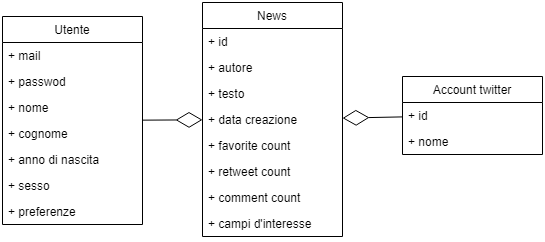
\includegraphics[height=5cm]{1.png}
\caption{Modello E/R}\label{fig:1}
\end{figure}

\subsubsection{Obiettivi funzionali di base}

Le funzionalità di base del sistema sono il reperimento dei tweet grazie alle API-twitter, tramite la realizzazione di un crawler, il salvataggio dei dati scaricati in un server così che possano poi essere elaborati e la realizzazione di un’interfaccia per permettere agli utenti di utilizzare l’applicazione.

Download dei dati e metadati

Indicizzazione

Profilazione utente

Ordinamento per interessi derivati dalla profilazione

Log in

Register

\subsubsection{Informazioni da prelevare}

Dai diversi account di Twitter prevediamo di prelevare news, ossia tweet, attraverso le api del social già ottenute. 
Ogni news sarà rappresentata da diversi campi come:

\begin{itemize}
\item ID: identificatore univoco della news. Twitter infatti associa ad ogni tweet un numero a 64 bit.

\item Autore: nome dell’autore della news. Twitter associa ad ogni tweet il nome dell’utente che lo ha postato.

\item Testo: il testo della news.

\item Data creazione: la data in cui l’utente ha postato il tweet.

\item favorite\_count: il numero riferito a quanti utenti lo hanno segnato come preferito.

\item retweet\_count: il numero riferito a quanti utenti lo hanno repostato.

\item reply\_count: il numero di quante persone hanno risposto/commentato il tweet
\end{itemize}

\subsubsection{Memorizzazione dei dati}

Le informazioni raccolte saranno memorizzate in una formattazione che permetta una gestione ottimale dei dati e metadati.

Come modello di organizzazione delle informazioni abbiamo pensato ad un metalinguaggio per la definizione di linguaggi di markup come XML. Esso infatti ci permette di raccogliere tutte le informazioni reperite dalle news in un unico documento suddiviso in singole news; ogni news sarà suddivisa a sua volta nei i vari campi di essa. 
La struttura del documento sarà dunque questa: 

\begin{figure}[h]
\centering
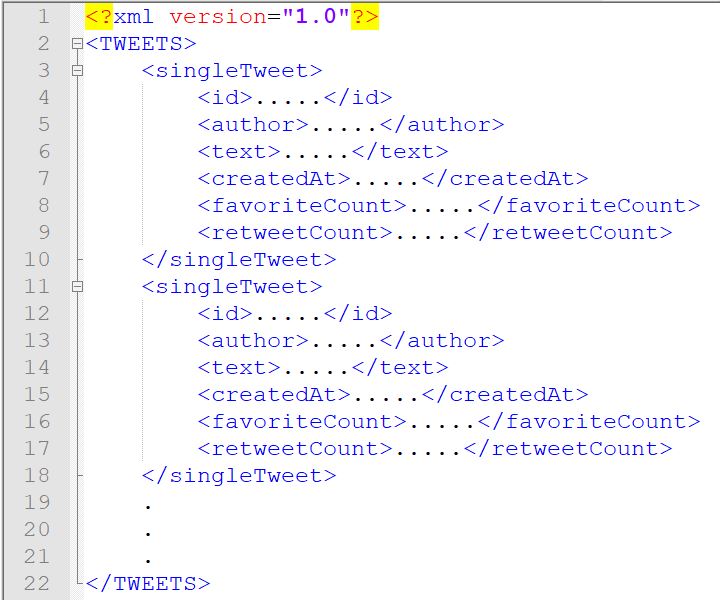
\includegraphics[height=8cm]{2.png}
\caption{Struttura XML}\label{fig:1}
\end{figure}

\subsubsection{Aggiornamento database}

Possiamo considerare il nostro database suddiviso in tre sezioni riguardanti rispettivamente le testate giornalistiche, gli utenti e le news. Queste tre sezioni prevediamo di aggiornarle con tempistiche differenti tra loro in quanto si hanno esigenze diverse per ognuna.

La parte del database riguardante le testate giornalistiche sarà quella che verrà aggiornata meno frequentemente in quanto prevediamo l'aggiunta o la rimozione di testate monitorando la loro attività su Twitter settimanalmente.

La parte delle news verrà invece aggiornata molto più frequentemente in quanto prevediamo il suo aggiornamento con una frequenza costante di 15 minuti. Con questa frequenza aggiungeremo le nuove news pubblicate della testate su Twitter nel nostro database.
Bisognerà considerare anche un periodo di permanenza della news all'interno del database. In quanto non consideriamo importante consigliare all'utente news troppo vecchie. Per questo motivo andremo a determinare una tempistica oltre la quale le news saranno considerate obsolete e quindi procederemo ad eliminarle dal database.

\subsection{Utenti e scenari di utilizzo}

Utenti registrati (con profilazione)

Utenti non registrati (senza profilazione)

Utenti amministratori

Modello di dominio: tutte entità più importanti espliciti ,non troviamo le parti architutturali. Si descrive il problema che si intende risolvere. Funzionalità, vincoli, entità

Modello dei dati memorizzazione, come vengono trattati e formato.

\newpage
\section{Requisiti Specifici}
\subsection{Requisiti Funzionali}
\textbf{\textit{Schema di descrizione dei requisiti}}

\textbf{Identificatore}: identificatore univoco del requisito.

\textbf{Descrizione}: rappresentazione verbale del requisito, inteso come narrazione del contesto di utilizzo e modalità di avvenimento dello stesso.

\textbf{Pre-condizione}: condizioni che devono essere verificate prima della funzione affinché possa essere eseguita correttamente.

\textbf{Input:} dati passati in ingresso alla funzione.

\textbf{Post-condizione}: condizioni che devono essere verificate dopo l’esecuzione della funzione.

\textbf{Output}: dati che la funzione in discussione restituisce in uscita. Indica il risultato prodotto dall’elaborazione.

\textbf{Priorità}: grado di rilevanza che ha la funzione rapportato al sistema. Ogni funzione sarà associata ad uno dei due gradi sottostanti:
\begin{itemize}
\item \textbf{Alta}
\item \textbf{Bassa}
\end{itemize}

\subsubsection{Requisiti dell'interfaccia}

\paragraph{Requisito funzionale 1: registrazione tramite mail}

\textbf{Identificatore}: rqs.mail.registration

\textbf{Descrizione:} se un utente vuole utilizzare la nostra applicazione dovrà innanzitutto utilizzare questa funzionalità. L’interfaccia grafica permetterà di registrarsi inserendo i dati come mail e password.

\textbf{Pre-condizione}: il sistema deve essere in esecuzione, l’utente deve essere nella pagina di registrazione, l’utente non deve essere ne loggato ne registrato.

\textbf{Input:} mail, password, nome, cognome, anno di nascita, sesso.

\textbf{Post-condizione}: viene creato un nuovo utente e i suoi dati salvati all’interno del server.

\textbf{Output}: messaggio di avvenuta registrazione.

\textbf{Priorità}: alta. Senza questa funzionalità l’utente non può iniziare ad utilizzare il sistema.

\paragraph{Requisito funzionale 2: registrazione tramite social}

\textbf{Identificatore}: rqs.social.registration

\textbf{Descrizione}: se un utente vuole utilizzare la nostra applicazione utilizzerà questa funzionalità. L’interfaccia grafica permetterà di registrarsi selezionando il social con il quale effettuare l’accesso.

\textbf{Pre-condizione}: il sistema deve essere in esecuzione, l’utente deve essere nella pagina di registrazione, l’utente non deve essere ne loggato ne registrato, deve possedere un account sul social selezionato.

\textbf{Input}: credenziali provenienti dal social selezionato.

\textbf{Post-condizione}: viene creato un nuovo utente e i suoi dati salvati all’interno del server.

\textbf{Output}: messaggio di avvenuta registrazione.

\textbf{Priorità}: alta. Senza questa funzionalità l’utente non può iniziare ad utilizzare il sistema.

\paragraph{Requisito funzionale 3: login}

\textbf{Identificatore}: rqs.login

\textbf{Descrizione}: tramite questa funzionalità un utente già registrato può effettuare l’accesso al sistema. Questo comporterà il caricamento dei dati e delle preferenze del suddetto utente.

\textbf{Pre-condizione}: il sistema deve essere in esecuzione, l’utente deve essere nella pagina di login, l’utente deve essere già registrato nel sistema e non deve essere loggato sul dispositivo che sta utilizzando.

\textbf{Input}: mail e password.

\textbf{Post-condizione}: viene eseguito l’accesso all’applicazione e vengono caricati i dati e le preferenze dell’utente.

\textbf{Output}: all’utente viene dato accesso alla schermata principale del sistema (schermata visualizzazione news).

\textbf{Priorità}: alta. Senza questa funzionalità sarebbe impossibile accedere all’applicazione e alle funzionalità di raccomandazione.

\paragraph{Requisito funzionale 4: prima profilazione}

\textbf{Identificatore}: rqs.first.profilation

\textbf{Descrizione}: dopo la procedura di registrazione viene mostrata all’utente una lista di interessi dalla quale può sceglierne alcuni. Tramite questa funzionalità viene effettuata la prima profilazione riguardante gli interessi dell’utente.

\textbf{Pre-condizione}: l’utente deve aver completato la procedura di registrazione, deve essere loggato e non deve aver effettuato ancora la prima profilazione.

\textbf{Input}: elementi scelti dalla lista di interessi.

\textbf{Post-condizione}: i dati di profilazione vengono salvati all’interno del server.

\textbf{Output}: all’utente viene dato accesso alla schermata principale del sistema (schermata visualizzazione news).

\textbf{Priorità}: alta. Per poter raccomandare le notizie, il sistema ha bisogno di conoscere gli interessi dell’utente.

\paragraph{Requisito funzionale 5: visualizzazione news}

\textbf{Identificatore}: rqs.news.visualization

\textbf{Descrizione}: quando l’utente entra nella pagina principale dell’applicazione, esso sarà in grado di visualizzare ed aprire le news che più gli interessano.

\textbf{Pre-condizione}: il sistema deve essere in esecuzione e l’utente deve essere loggato.

\textbf{Input}:  lista di news.

\textbf{Post-condizione}: nessuna.

\textbf{Output}: vengono visualizzate le news nella pagina principale del sistema.

\textbf{Priorità}: alta. Senza questa funzionalità l’utente non potrebbe leggere alcuna news.

\paragraph{Requisito funzionale 6: ordinamento di default (rilevanza)}

\textbf{Identificatore}: rqs.news.sorting.relevance

\textbf{Descrizione}: quando l'utente accede alla pagina principale dell'applicazione le news saranno ordinate secondo la rilevanza ottenuta tramite la profilazione dell'utente. Questo è l'ordinamento di default.

\textbf{Pre-condizione}: il sistema deve essere in esecuzione e l'utente deve essere loggato.

\textbf{Input}: lista di news.

\textbf{Post-condizione}: nessuna.

\textbf{Output}: l'utente visualizza le news ordinate per rilevanza rispetto ai suoi interessi.

\textbf{Priorità}: alta. Senza questa funzionalità l'utente all'utente verrebbero mostrate notizie non per forza rilevanti rispetto ai suoi interessi.

\paragraph{Requisito funzionale 7: ordinamento per data}

\textbf{Identificatore}: rqs.news.sorting.date

\textbf{Descrizione}: quando l'utente accede alla pagina principale dell'applicazione avrà la possibilità, tramite l'utilizzo di un menù di opzioni, di ordinare le news in maniera differente rispetto a quella di default (Requisito funzionale 6), ordinandole per data di pubblicazione.

\textbf{Pre-condizione}: il sistema deve essere in esecuzione e l'utente deve essere loggato.

\textbf{Input}: lista di news.

\textbf{Post-condizione}: nessuna.

\textbf{Output}: l'utente visualizza le news ordinate per data di pubblicazione.

\textbf{Priorità}: bassa. Non è un requisito fondamentale per il funzionamento base del sistema.

\paragraph{Requisito funzionale 8: ordinamento per like}

\textbf{Identificatore}: rqs.news.sorting.like

\textbf{Descrizione}: quando l'utente accede alla pagina principale dell'applicazione avrà la possibilità, tramite l'utilizzo di un menù di opzioni, di ordinare le news in maniera differente rispetto a quella di default (Requisito funzionale 6), ordinandole per numero di like.

\textbf{Pre-condizione}: il sistema deve essere in esecuzione e l'utente deve essere loggato.

\textbf{Input}: lista di news.

\textbf{Post-condizione}: nessuna.

\textbf{Output}: l'utente visualizza le news ordinate per numero di like.

\textbf{Priorità}: bassa. Non è un requisito fondamentale per il funzionamento base del sistema.

\paragraph{Requisito funzionale 9: ordinamento per retweet}

\textbf{Identificatore}: rqs.news.sorting.retweet

\textbf{Descrizione}: quando l'utente accede alla pagina principale dell'applicazione avrà la possibilità, tramite l'utilizzo di un menù di opzioni, di ordinare le news in maniera differente rispetto a quella di default (Requisito funzionale 6), ordinandole per numero di volte che è stata retweettata.

\textbf{Pre-condizione}: il sistema deve essere in esecuzione e l'utente deve essere loggato.

\textbf{Input}: lista di news.

\textbf{Post-condizione}: nessuna.

\textbf{Output}: l'utente visualizza le news ordinate per numero di retweet.

\textbf{Priorità}: bassa. Non è un requisito fondamentale per il funzionamento base del sistema.

\paragraph{Requisito funzionale 10: ordinamento per commenti}

\textbf{Identificatore}: rqs.news.sorting.comments

\textbf{Descrizione}: quando l'utente accede alla pagina principale dell'applicazione avrà la possibilità, tramite l'utilizzo di un menù di opzioni, di ordinare le news in maniera differente rispetto a quella di default (Requisito funzionale 6), ordinandole per numero di commenti.

\textbf{Pre-condizione}: il sistema deve essere in esecuzione e l'utente deve essere loggato.

\textbf{Input}: lista di news.

\textbf{Post-condizione}: nessuna.

\textbf{Output}: l'utente visualizza le news ordinate per numero di commenti.

\textbf{Priorità}: bassa. Non è un requisito fondamentale per il funzionamento base del sistema.

\paragraph{Requisito funzionale 11: aggiornamento news}

\textbf{Identificatore}: rqs.news.refresh

\textbf{Descrizione}: l'utente all'interno della pagina principale dell'applicazione avrà la possibilità di aggiornare l'elenco di news mostrate. Questo permetterà di mantenere costantemente aggiornata la pagina principale con le news più recenti.

\textbf{Pre-condizione}: il sistema deve essere in esecuzione e l'utente deve essere loggato.

\textbf{Input}: nessuno.

\textbf{Post-condizione}: vengono inserite nuove news all'interno di quelle gestite dal sistema.

\textbf{Output}: il sistema restituirà un messaggio di avvenuto aggiornamento.

\textbf{Priorità}: alta. Senza questa funzionalità non ci sarebbe la possibilità di aggiornare le news.

\paragraph{Requisito funzionale 13: logout}

\textbf{Identificatore}: rqs.logout

\textbf{Descrizione}: l'utente ha la possibilità di effettuare il logout dall'applicazione.

\textbf{Pre-condizione}: il sistema deve essere in esecuzione e l'utente deve essere loggato.

\textbf{Input}: nessuno.

\textbf{Post-condizione}: l'utente viene disconnesso dall'applicazione.

\textbf{Output}: viene visualizzato un messaggio di avvenuta disconnessione.

\textbf{Priorità}: alta. Senza questa funzione l'utente non sarebbe in grado di disconnettersi.

\subsubsection{Requisiti del server}

\paragraph{Aggiornamento preferenze utente}

\textbf{Identificatore}: rqs.update.preferences

\textbf{Descrizione}: Il sistema sarà in grado di aggiornare automaticamente le preferenze di ogni singolo utente in base alle news che questo apre.

\textbf{Pre-condizione}: il sistema deve essere in esecuzione.

\textbf{Input}: news aperte dagli utenti.

\textbf{Post-condizione}: aggiornamento della profilazione utente.

\textbf{Output}: nessuno.

\textbf{Priorità}: alta. Senza questa funzione il sistema non sarebbe in grado di aggiornare la profilazione degli utenti in base alle news che questi leggono.

\paragraph{Crawling tramite api-twitter}

\textbf{Identificatore}: rqs.crawling

\textbf{Descrizione}: il sistema è in grado di scaricare le news da twitter grazie all'utilizzo delle sue API.

\textbf{Pre-condizione}: il sistema deve essere in esecuzione e deve avere accesso ai dati twitter tramite token valido.

\textbf{Input}: elenco di account twitter da cui scaricare dati.

\textbf{Post-condizione}: vengono scaricati e salvati i dati nel server.

\textbf{Output}: nessuno.

\textbf{Priorità}: alta. Senza questa funzione non sarebbe possibile reperire news.

\paragraph{Indicizzazione dati news}

\textbf{Identificatore}: rqs.indexing

\textbf{Descrizione}: il sistema sarà in grado di indicizzare le news presenti all'interno del server.

\textbf{Pre-condizione}: il sistema deve essere in esecuzione e devono essere presenti news salvate nel server.

\textbf{Input}: lista news.

\textbf{Post-condizione}: i dati all'interno del server vengono elaborati per poter essere interpretati e utilizzati in futuro.

\textbf{Output}: nessuno.

\textbf{Priorità}: alta. Senza questa funzionalità il sistema non sarebbe in grado di organizzare e gestire i dati.

\paragraph{Algoritmo di raccomandazione}

\textbf{Identificatore}: rqs.recommendation

\textbf{Descrizione}: il sistema utilizzerà un algoritmo di raccomandazione che gestirà le news e le preferenze degli utenti per mostrare news rilevanti all'interesse dell'utente.

\textbf{Pre-condizione}: il sistema deve essere in esecuzione e devono essere presenti news indicizzate salvate nel server.

\textbf{Input}: lista news e preferenze utente.

\textbf{Post-condizione}: vengono riorganizzate le news in base alle preferenze di ogni singolo utente.

\textbf{Output}: nessuno.

\textbf{Priorità}: alta. Senza questa funzione il sistema non sarebbe in grado di raccomandare news.

\paragraph{Aggiornamento automatico news}

\textbf{Identificatore}: rqs.automatic.update

\textbf{Descrizione}: il sistema effettuerà un aggiornamento periodico dei dati utilizzati in modo da mantenere aggiornato il database. Ciò implicherà un'esecuzione periodica delle funzioni espresse nei requisiti 3.1.2.2, 3.1.2.3 e 3.1.2.4.

\textbf{Pre-condizione}: il sistema deve essere in esecuzione.

\textbf{Input}: nessuno.

\textbf{Post-condizione}: vengono scaricate nuove news, indicizzate e organizzate in base alle preferenze di ogni singolo utente.

\textbf{Output}: nessuno.

\textbf{Priorità}: alta. Permette al sistema di aggiornarsi periodicamente.


\subsection{Requisiti non funzionali}
\subsubsection{Disponibilità/affidabilità}

Il sistema deve essere disponibile 24 ore al giorno, 365 giorni all'anno. Nell’arco dell'anno è tollerabile avere un numero di interruzioni del servizio non superiori a 10. Queste interruzioni comprendono sospensioni del servizio causate da manutenzione programmata o da guasto improvviso. Ognuna di queste interruzioni non dovrà superare le due ore.

\subsubsection{Sicurezza}

I dati confidenziali dovranno essere protetti.

\subsubsection{Portabilità}

L'applicazione dovrà essere supportata da un qualsiasi browser.

\subsubsection{Usabilità}
\subsubsection{Scalabilità}
\subsubsection{Vincoli di progettazione}
\subsubsection{Performance}


 
\end{document}


